\documentclass[10pt]{article}

\usepackage{changepage}
\usepackage{amsmath}
\usepackage{amsfonts}
\usepackage{amssymb}
\usepackage{url}
\usepackage{indentfirst}
\usepackage{hanging}
\usepackage{titlesec}
\usepackage[document]{ragged2e}
\usepackage{hyperref}
\usepackage{minted}
\usepackage{graphicx}

\setlength{\parindent}{0pt}
\setlength{\RaggedRightParindent}{0pt}
\setlength{\parskip}{0pt}

\renewcommand{\labelitemi}{\(\hookrightarrow\)}
\setlength{\itemsep}{0pt}
\titleformat{\section}{\normalfont}{\thesection}{1em}{}

\title{web design in c++26}
\date{2026-08-01}

\begin{document}

\maketitle 

\begin{center}
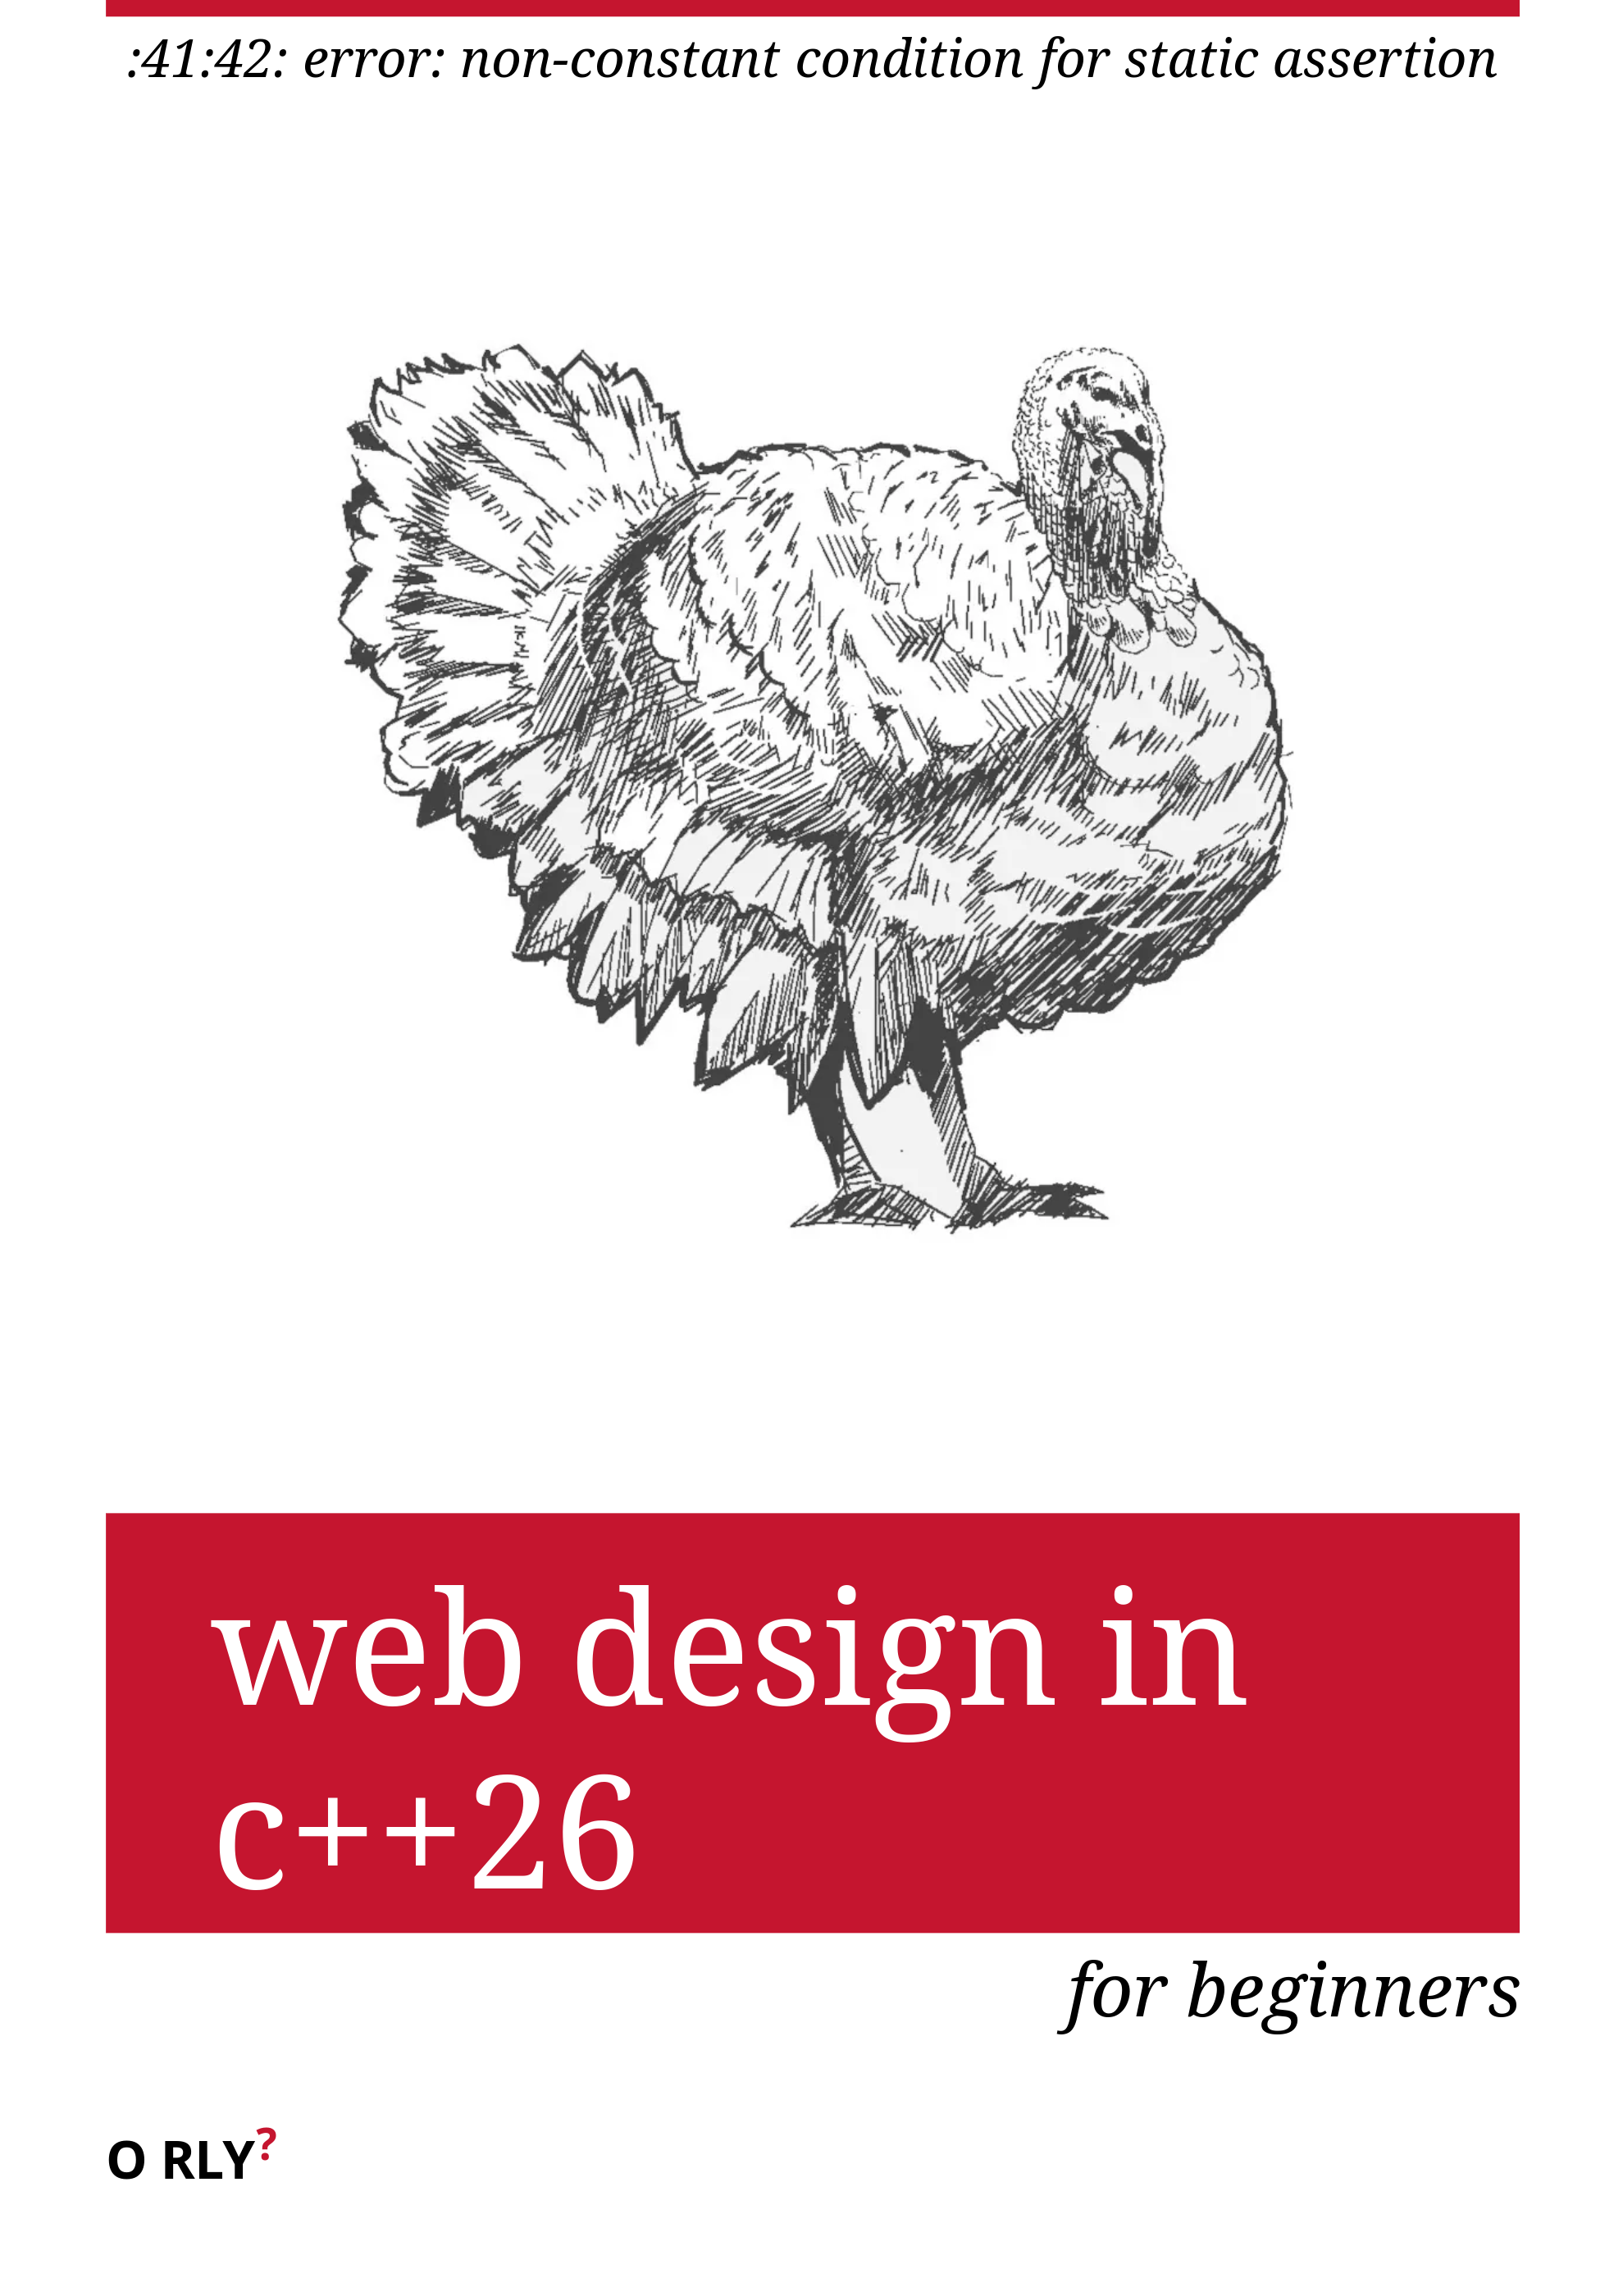
\includegraphics[width=0.9\linewidth]{./book_cover.png}
\end{center}

So, the problem is that I don't really like writing HTML by hand, but I feel in this era of technology an overwhelming compulsion to make things with my hands. The thing I wanted was simple --- a way to generate the featureless, dry homepage of this site from the posts that I've written --- and the result, I think, is elegant:

\begin{minted}{cpp}
inline constexpr post site_posts[]{
    { "web design in c++26", std::chrono::August/1/2026, R"(or, <c style="font:10pt monospace">/usr/include/c++/16/span: In instantiation of </c>)" },
};

static constexpr auto index_entry(const post& p) {
    using namespace ml;
    using namespace css;
    using namespace std::string_view_literals;
 
    return a{ $style(css::$color = "inherit", $text_decoration = "none"), $href = p.encoded_name,
            ml::div{ $id = p.encoded_name, $style = post_item_style(),
                span{ $style($font_size = "1.25em", $font_weight = "bold"), p.hed },
                span{ $style(css::$color = "gray", $white_space = "nowrap"), p.date },
                ml::div{ $style = post_subhed_style(), p.subhed }
        }
    };
}

template <class = void> constexpr auto post_list() {
    using namespace ml;
    using namespace css;
    using namespace std::string_view_literals;

    const auto& [...posts] = site_posts;

    return ml::div { $style($text_align = "left", $padding = "1em"),
        ml::div{ $style($padding = "2pt", $border_bottom = "1pt solid lightgray", css::$height = "1pt"), ""sv },
        index_entry(posts)...
    };
}
\end{minted}

\section*{the best program is one that does nothing at all}

Let's say our goal was the nebulous ``make a webpage in C++.'' There are plenty of libraries that would technically allow one to programmatically construct an HTML document (and if that's what you want, \href{https://github.com/zeux/pugixml}{pugixml} is a good one), but for our purposes, that's overkill. The text of this website is static, and we only need to regenerate our homepage occasionally, after making manual changes to the posts on the site. So, what if we instead made C++ code constructs that mirrored those in the HTML specification? 

For example, to represent a link, the HTML element \verb|<a>| element allows the attribute \verb|href|, so we could represent it in C++ like: 
\begin{minted}{cpp}
struct a {
    std::string href;
};
\end{minted}
and imitate the HTML syntax with designated initializers, like \mintinline{cpp}{a link{ .href = "#" }}. 

But the \mintinline{html}|<a>| element permits far more attributes than just \mintinline{html}|href| --- and, what's worse, some of these attributes have names which aren't legal C++ identifiers (like \mintinline{cpp}|class|) so our C++ type would have to look more like:
\begin{minted}{cpp}
struct a {
    // attributes common to all elements
    attribute<"title", std::string_view> title;
    attribute<"lang", std::string_view> lang;
    attribute<"translate", bool> translate;
    attribute<"dir", std::string_view> dir;
    attribute<"hidden", std::variant<bool, double, std::string_view>> hidden;
    attribute<"inert", bool> inert;
    attribute<"innerText", std::string_view> innerText;
    attribute<"outerText", std::string_view> outerText;
    attribute<"class", std::string_view> className;
    attribute<"id", std::string_view> id;

    // attributes specific to anchor elements
    attribute<"href", std::string_view> href;
    attribute<"target", std::string_view> target;
    attribute<"download", std::string_view> download;
    attribute<"ping", std::string_view> ping;
    attribute<"rel", std::string_view> rel;
    attribute<"relList", ::ht::unimplemented> relList;
    attribute<"hreflang", std::string_view> hreflang;
    attribute<"type", std::string_view> type;
    attribute<"text", std::string_view> text;
    attribute<"referrerPolicy", std::string_view> referrerPolicy;

    // and so on
};
\end{minted}

Very quickly, we've ended up with a comically large and unwieldy object that must be large enough to contain the values for \textit{all} of these attributes, even if we never use them (which is usually the case). Now, practically this wouldn't be a problem, but it would be deeply unsatisfying. Worse, designated initializers can only be specified in the order that the corresponding data members are defined, so \mintinline{cpp}|a link{ .href="#" .id="anchor" }| would be ill-formed. 

Famously, C++ is philosophically oriented towards the ``zero-overhead principle,'' that the language should not provide facilities which would incur a greater cost (in whatever sense) than the programmer writing the same code by hand. Now, it wouldn't make sense to measure ourselves against writing twenty lines of HTML by hand, but we can reasonably expect our construct not to waste space in such a way.

We can interpret the zero-overhead principle in an even more extreme way. If the best program that completes our task is the one that does it the most efficiently (as fast a possible, with as few resources as possible) then the best possible program is one that does nothing at all. C++ is known for its compile-time features, from template metaprogramming to \verb|constexpr| code, introduced with C++11, to static reflection, introduced just now in C++26. With this in mind, we can also ask that our program accomplish as much of its work at compile-time as possible. 

{\Large\bfseries hell is empty, and all the \mintinline{cpp}|std::meta::define_aggregate|s are here}

So, back to what we have: \mintinline{cpp}|a{ $href = "#", "click here!"sv }|.

\begin{minted}{cpp}
template <class ...A> struct a: public element<a<A...>> {
    constexpr a(A&& ...a): a::element{ std::move(a)... } { }
};
\end{minted}
The value of the expression \mintinline{cpp}|$href = "#"| is an \textit{aspect}. \mintinline{cpp}|$href| is an \textit{aspect generator}, declared as 
\begin{minted}{cpp}
inline constexpr aspect_generator<^^std::string_view, "href"> a;
\end{minted} 

When we write \mintinline{cpp}|$href = "#"|, we're really just abusing the copy assignment operator:
\begin{minted}{cpp}
template <std::meta::info VTp, static_string Name, auto Tag = []{}> struct aspect_generator { 
    // ...
    template <class ...Args> constexpr decltype(auto) operator()(Args&& ...args) const {
        typename[:VTp:] r{ std::forward<Args>(args)... };
        return aspect<decltype(r), aspect_generator>{ std::move(r) };
    }

    template <class T> constexpr decltype(auto) operator=(T&& t) const {
        return this->operator()(std::forward<T>(t));
    }
    // ...
\end{minted}
Of all this nonsense, \mintinline{cpp}|typename[:VTp:] r{ std::forward<Args>(args)... };| might be my favorite. In the example, where \mintinline{cpp}|VTp| is the type reflection \mintinline{cpp}|^^std::string_view|, \mintinline{cpp}|typename[:VTp:]| is just \mintinline{cpp}|std::string_view|. But \mintinline{cpp}|VTp| \textit{doesn't have to be a type reflection}. 

Here's an example from another project using the same code. When printing formatted output to the terminal, one can use \(256\)-color mode, where the first \(16\) colors are set by the user's terminal theme and the remaining \(240\) are a fixed color palette, or the direct mode, where one can specify a \(24\)-bit RGB color. While most color terminals will support the former, usually only graphical terminals will support the latter. 

\begin{minted}{cpp}
enum color_mode { XTERM_256COLOR = 8, DIRECT = 24 };

template <color_mode Mode> struct color;
// color<XTERM_256COLOR> holds one uint8_t, while color<DIRECT> holds three
// ...
// deduction guides:
color(uint8_t) -> color<XTERM_256COLOR>;
color(uint8_t, uint8_t, uint8_t) -> color<DIRECT>;

inline constexpr aspect_generator<^^color, "fg"> $fg;
inline constexpr aspect_generator<^^color, "bg"> $bg;
\end{minted}
Now, we can write either \mintinline{cpp}|$fg(1)| for the \(256\)-color red or \mintinline{cpp}|$fg(255, 0, 0)| for direct-color primary red with a uniform syntax! Inside the aspect generator, \mintinline{cpp}|VTp| is a reflection of the \textit{template-name} \mintinline{cpp}|color|, so after splicing, we get \mintinline{cpp}|color r{ std::forward<Args>(args)... }|. Here, \mintinline{cpp}|color| is a \textit{placeholder-type} and, because of our user-defined deduction guides, is deduced to be either \mintinline{cpp}|color<XTERM_256COLOR>| or \mintinline{cpp}|color<DIRECT>| depending on the number of arguments.\footnote{When I first tried this, GCC didn't parse it correctly, but they kindly \href{https://gcc.gnu.org/bugzilla/show_bug.cgi?id=124706}{fixed it for me}.}

Constructed with an argument of type \mintinline{cpp}{aspect<std::string_view, aspect_generator<(...)>>}, we trigger a specialization of \mintinline{cpp}{element<A...>} and its base classes, \mintinline{cpp}{with_aspects<A...>} and \mintinline{cpp}{with_children<A...>}. We encounter the \mintinline{cpp}{consteval} block of each:

\begin{minted}{cpp}
template <class... A> struct with_aspects_impl {
    struct aspects_impl;
    struct children_impl;

    consteval {
        std::vector<std::meta::info> mems;
        std::vector<std::meta::info> child_types;

        // this was originally an expansion statement but it causes a crash in clangd that i don't understand so we're
        // back to doing it this way.
        [&]<std::size_t ...Is>(std::index_sequence<Is...>){
            ([&]<std::size_t I, class T>(){
                static constexpr auto a = ^^T;

                if constexpr (is_aspect_type(a)) {
                    mems.push_back(std::meta::data_member_spec(a, { .name = "_" + std::string{ aspect_name<typename[:a:]> } }));
                } else if constexpr (is_type(a)) {
                    child_types.push_back(std::meta::data_member_spec(a, { .name = child_name<I, a>() }));
                }
            }.template operator()<Is, A>(), ...);
        }(std::make_index_sequence<sizeof...(A)>{ });

        define_aggregate(^^aspects_impl, mems);
        define_aggregate(^^children_impl, child_types);
    }
};
\end{minted}

% change this, the example should be <a href="$">click here</a>

The specialization of \mintinline{cpp}{a} we have defined two new types, looking something like:

\begin{minted}{cpp}
struct with_aspects_impl<aspect<std::string_view, aspect_generator</*...*/>>> {
    struct aspects_impl {
        std::string_view _href;
    };

    struct children_impl{
        std::string_view string_view0;
    };
}
\end{minted}

Both \mintinline{cpp}|aspects_impl| and \mintinline{cpp}|children_impl| are public bases of our specialization of \mintinline{cpp}|a|. In the constructor of \mintinline{cpp}|element<El<A...>>|, we iterate over the arguments:
\begin{minted}{cpp}
    template <class T, std::size_t I> constexpr void initialize(T&& t) {
        constexpr auto info = ^^T;
        if constexpr (is_aspect_type(info)) {
            constexpr auto generator_info = get_generator_info(info);
            std::construct_at(std::addressof(this->[:aspect_info<typename[:generator_info:]>():]), std::forward<T>(t));
        } else {
            std::construct_at(std::addressof(this->[:children_in()[child_index_from_raw_index<I>()]:]), std::forward<T>(t));
        }
    }

public:
    constexpr element(A... args) {
        template for (constexpr auto I : detail::index_range<sizeof...(A)>) {
            this->template initialize<A...[I], I>(std::forward<A...[I]>(args...[I]));
        }
    }
\end{minted}

If \mintinline{cpp}|T| is a specialization of \mintinline{cpp}|aspect|, we initialize the corresponding data member in the \mintinline{cpp}|with_aspects_impl::children_impl| base class, which can be determined based on the index of the argument. Otherwise, we initialize the corresponding member of the \mintinline{cpp}|aspects_impl| base. Currently, the aspect members are identified by name, but this should change in a later version. 

\section*{tying up loose ends except the ends are all loose and i'm not even sure if they're ends at all}

One remaining problem is that some of the strings we want to use as aspect names aren't valid C++ identifiers, such as CSS property names which contain a ``-''. Although we can change the name of the identifier, we need to remember the original, illegal name \textit{and retrieve it having only an} \mintinline{cpp}|aspect_generator| \textit{type}. Underlying this is a more general desire --- we might want to have some arbitrary annotation that could be applied to aspect generators and then retrieved later; something like:
\begin{minted}{cpp}
inline constexpr [[=property_name("font-weight")]] aspect_generator<^^std::string_view, "font_weight"> $font_weight;
\end{minted}

The problem is that we can only apply an annotation to the \textit{declaration} \mintinline{cpp}|$font_weight|, so we would need to store a reflection of that object alongside every \mintinline{cpp}|aspect| it generates. This isn't possible because we need to generate those aspects from the \mintinline{cpp}|aspect_generator</**/>::operator=| function, and we can't reflect the \mintinline{cpp}|this| pointer. This feels like an absurd problem to have, but our solution might be more absurd.

Here's the actual declaration for \mintinline{cpp}|$font_weight|:
\begin{minted}{cpp}
inline constexpr aspect_generator<^^std::string_view, "font_weight", [][[=format_name("font-weight")]]{}> $font_weight;
\end{minted}

Were I asked why I did this, I could only say it was an artistic inspiration, because I'm certain there are better ways. But --- what we've done is added another template parameter to \mintinline{cpp}|aspect_generator| that defaults to a trivial lambda \mintinline{cpp}|[]{}|. Now, we can access the annotations on that lambda from a reflection of the \mintinline{cpp}|aspect_generator| specialization. This also solves a more philosophical problem --- because each declaration of a lambda is guaranteed to be a unique type, each instantiation of an \mintinline{cpp}|aspect_generator| is now a unique template specialization, even if the lambda parameter appears the same. I believe this will aid in removing some of the dependence on string identifiers for aspect generators, but that's a problem for future me to solve. 

Currently, we use \mintinline{cpp}|std::format| to print HTML to a file, which works fine, but is a little unsatisfying. Although presently the \mintinline{cpp}|std::format| library isn't usable in constant expressions, its \mintinline{cpp}|constexpr|ification has been accepted as \href{https://www.open-std.org/jtc1/sc22/wg21/docs/papers/2025/p3391r2.html}{P3391} for C++29, and has already been \href{https://gcc.gnu.org/pipermail/gcc-patches/2026-June/718980.html}{implemented for the upcoming GCC 17}. Once it's released, and this is the dream, possibly we can generate a website in C++ without ever executing the program. 

\end{document}

